\section{Versuchsaufbau und Versuchsdurchführung}

\begin{flushleft}
    Der Versuch wird wie in Abbildung \ref{Abbildung4} zu sehen aufgebaut.
\end{flushleft}

\begin{figure}[H]
    \centering
    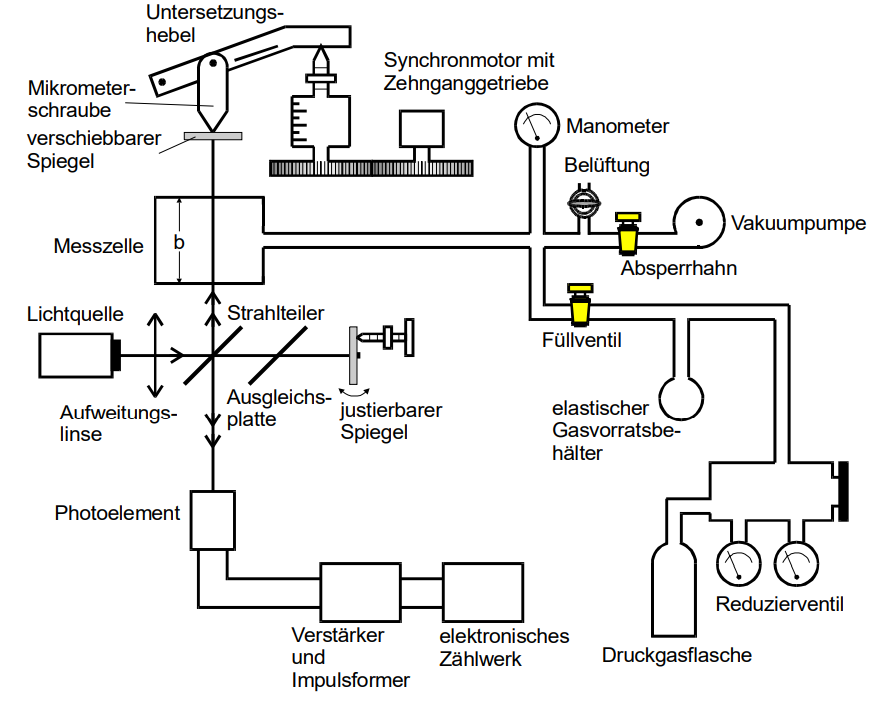
\includegraphics[height=80mm]{bilder/Ab4.png}
    \caption{Schematische Darstellung der kompletten Messapparatur \cite{a1}. \label{Abbildung4} }
\end{figure}

\begin{flushleft}
    Nach dem Aufbau der Versuchs muss das Michelson-Interferometer justiert werden. 
    Dafür wird die Lichtquelle, welche hierbei ein Laser ist, angestellt und an dem Regler des justierbaren Spiegels so eingestellt das beide Strahlen übereinander liegen.
    Dabei muss darauf geachtet werden, dass diese überliegenden Strahlen auf das Loch des Photoelements trifft, damit die Messwerte richtig aufgenommen werden können.
\end{flushleft}

\subsection{Bestimmung der Wellenlänge}

\begin{flushleft}
    Um die Wellenlänge des Lasers zu bestimmen wird der verschiebbare Spiegel mit einer Mikrometerschraube, welche sich durch ein Synchronmotor verstellen lässt, verschoben.
    Der Motor wird so eingestellt, dass der Spiegel durch die Mikrometerschraube nicht zu schnell verstellt wird, da das Photoelement sonst nicht alle Impulse ausreichend erkennen kann.
    Es wird bei einer beliebigen Verschiebung angefangen, bevorzugt $5\,\unit{\milli\meter}$ aufwärts. 
    Danach wird der Impulszähler zurückgesetzt und der Motor so eingestellt, dass sich die Verschiebung verkleinert.
    Der Motor wird gestoppt wenn der Impulszähler 2000 Impulse gemessen hat und die Verschiebung wird erneut aufgenommen.
    Dies wird acht mal wiederholt für die selbe Startverschiebung. 
\end{flushleft}

\subsection{Bestimmung des Brechungsindexes von Luft}

\begin{flushleft}
    Um den Brechungsindex von Luft zu bestimmen wird der verschiebbare Spiegel einmal fest eingestellt und die Messzelle evakuiert.
    Evakuiert wird die Messzelle mit einer Vakuumpumpe.
    Dabei wird der Druck, der in der evakuierten Messzelle herrscht, aufgenommen, der Impulszähler zurückgesetzt und langsam durch das Ventil an der Vakuumpumpe Luft in die evakuierte Messzelle eingelassen.
    Wenn in der Messzelle wieder Normaldruck herrscht wird die Zählrate notiert.
    Dies wird fünf mal wiederholt.
\end{flushleft}